\section{Application Interface}

\subsection{Overview}
The application window, Figure 1, is divided into a tool bar and two main regions: a central analysis area with two panels A and B, and a right sidebar with the database and recordings management tools.

\begin{figure}[h]
	\centering
	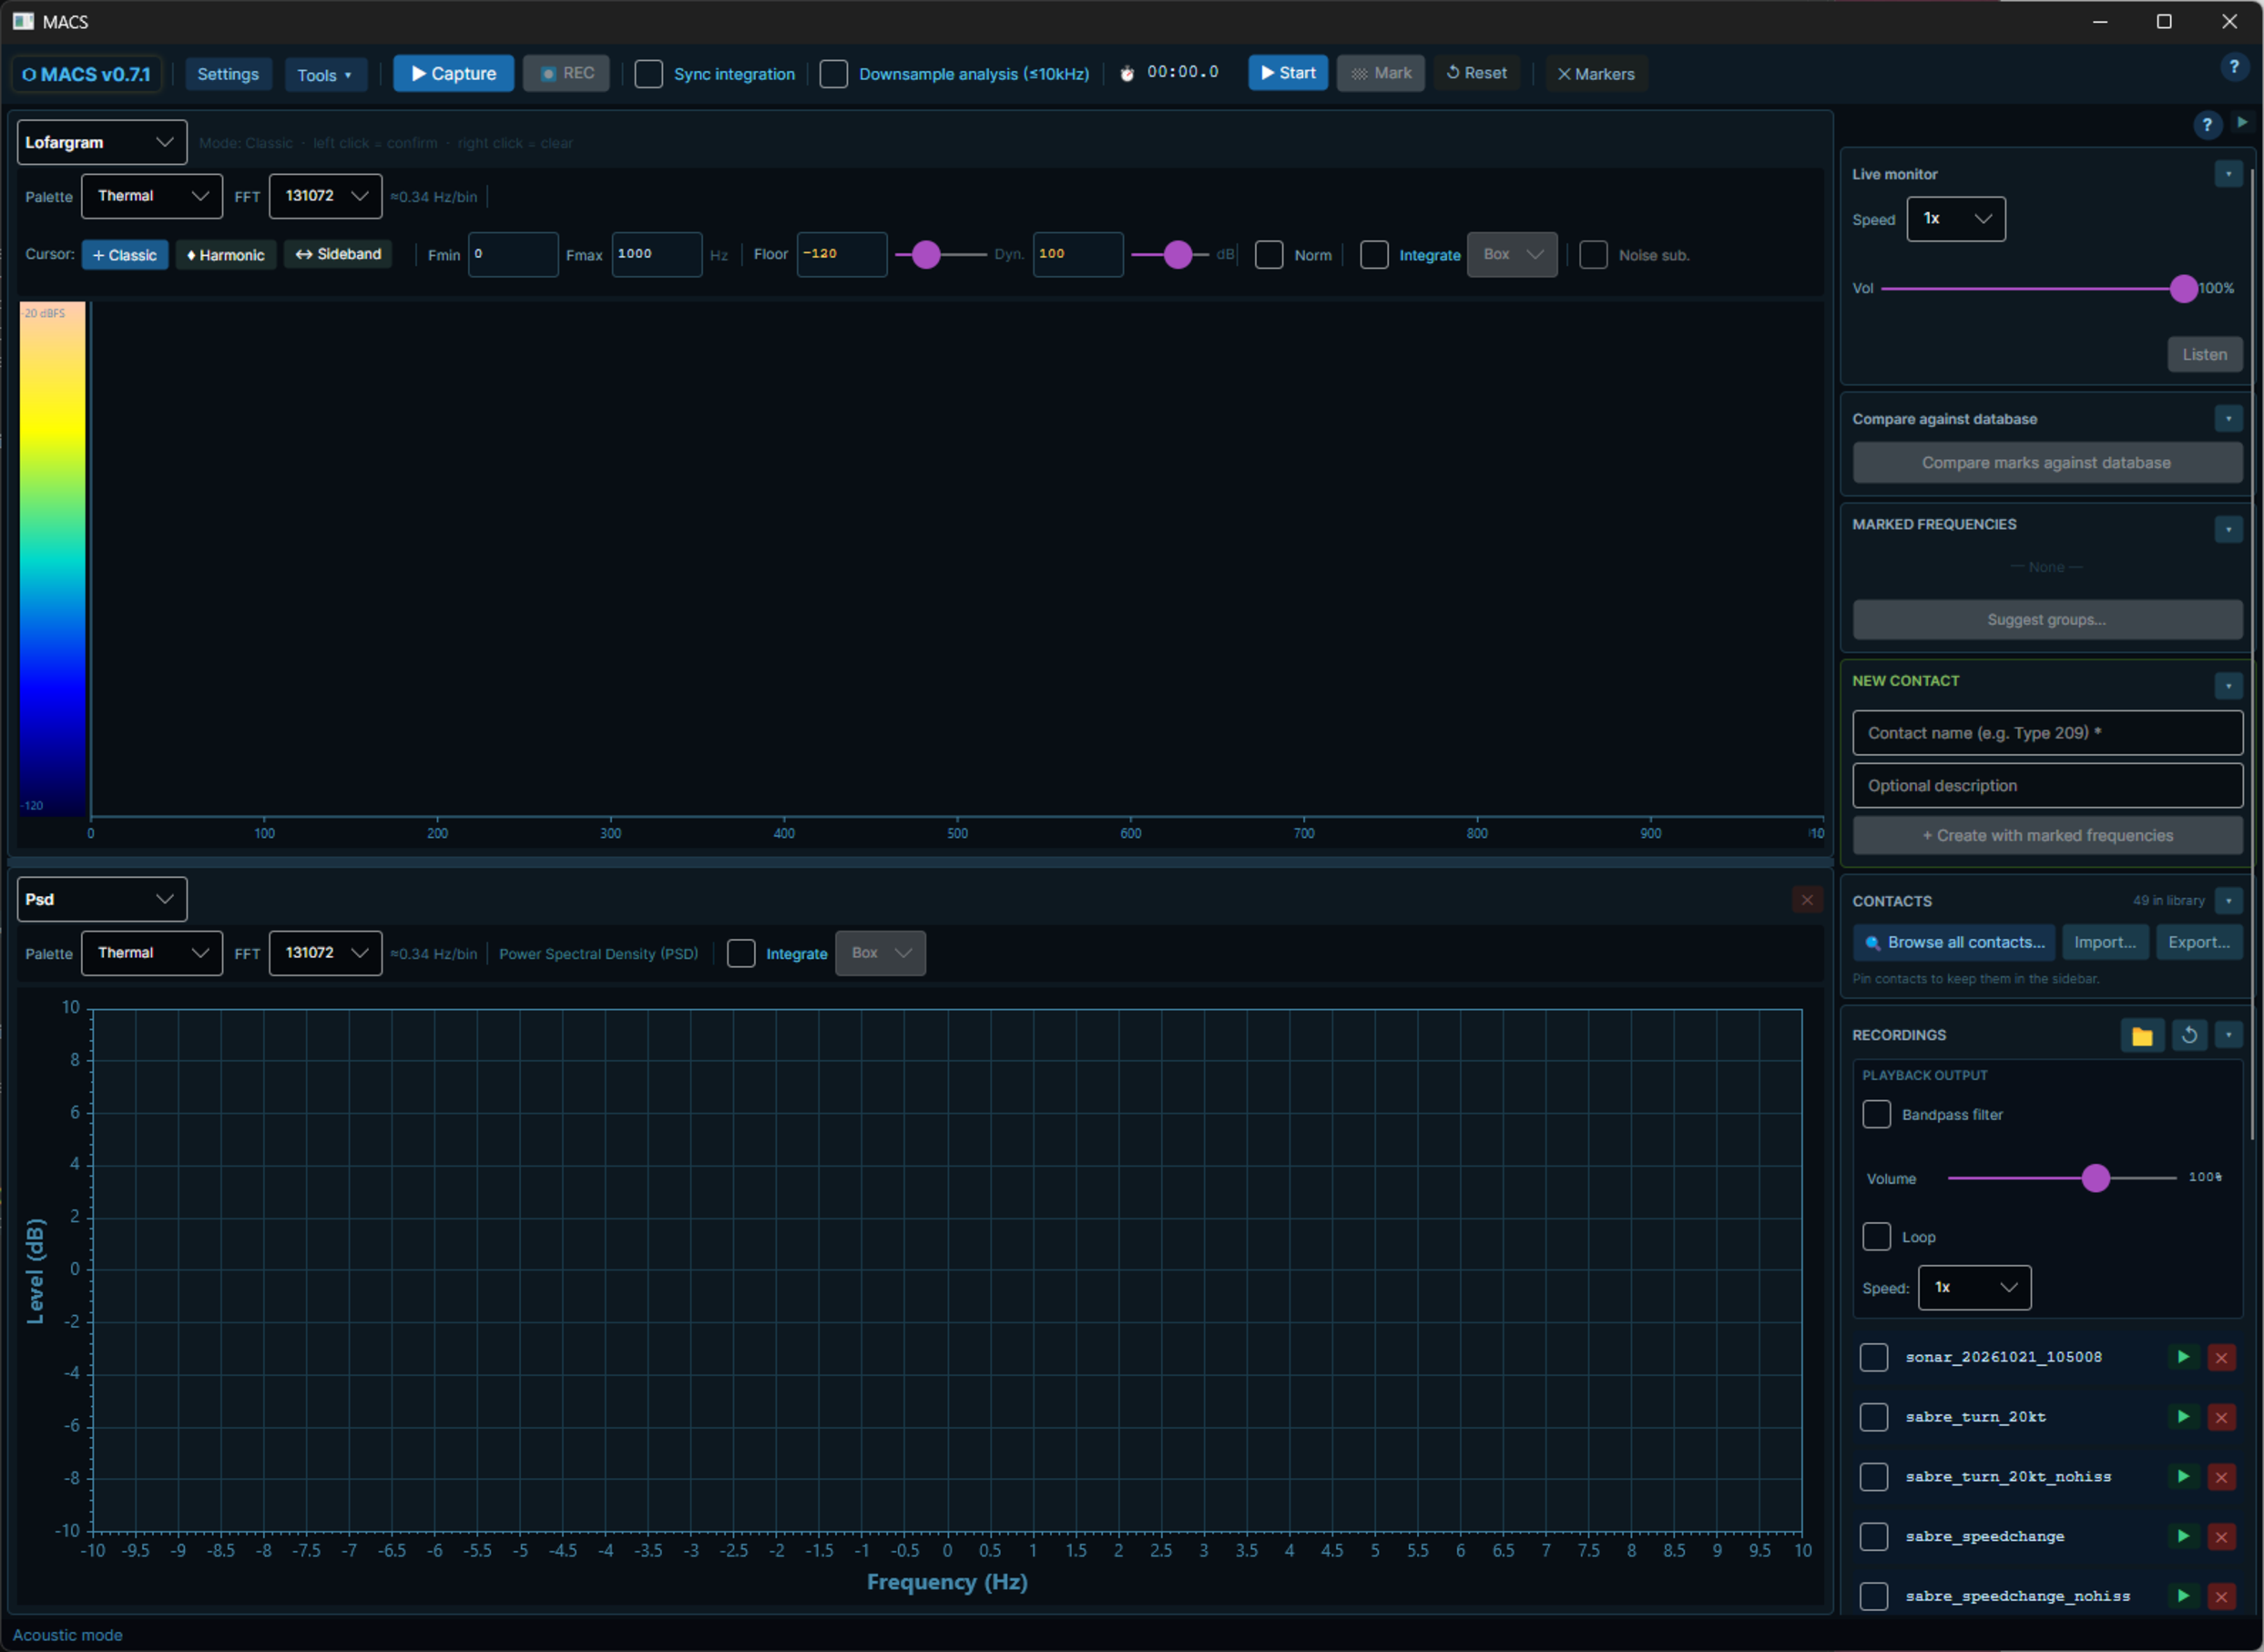
\includegraphics[width=345px]{../img/actuals/MACS.pdf}
	\caption{MACS Application Interface}
\end{figure}

\subsection{The Title Bar}

The title bar (Figure 2) has options to control the audio source, to start audio capture, manipulate the behaviours of Panel A and B, limit sample analysis and to enable recording for off line analysis. The title bar contains the following global controls:

\begin{figure}[h]
	\centering
	
\includegraphics[width=450px]{../img/actuals/topbar.pdf}
	\caption{The Title Bar}
\end{figure}

\begin{compactitem}
    \item \textbf{MACS Version:} Application version.
    \item \textbf{Settings:} View the settings panel.
    \item \textbf{Tools:} Dropdown to select tools.
    \item \textbf{Capture:} Starts live audio capture from the system (microphone / loopback).
    \item \textbf{REC:} Records the current capture to a WAV file in the recordings folder.
    \item \textbf{Sync Integration:} Synchronises settings between Panel A and B.
    \item \textbf{Downsample Analysis ($\le$ 10kHz):} Limits FFT / DEMON / Cepstrum / ACF to content $\le$ 10kHz.
    \item \textbf{Timer:} A useful timer with Start/Stop/Mark/Reset functionality.
    \item \textbf{Markers:} Toggles setting and deleting active frequency marker.
    \item \textbf{?:} On-screen guide to basic functionality, hover over options for on-screen guides.
\end{compactitem}

Hovering the mouse pointer over any of the controls will pop up an information box with more detail about it.
\pagebreak
\subsection{Main Panel - Central Analysis Area}

The main panel (Figures 3 and 4) hosts two display panels A and B. Both panels display a user select-able visual representations of the sound analysis performed by the application. Each panel has its own toolbar strip immediately above it, containing

\begin{compactitem}
    \item Content dropdown
    \item Palette selector
    \item FFT size
    \item Integrate
\end{compactitem}

In addition panel A has the following:

\begin{compactitem}
    \item Full cursor and display parameter row (Fmin / Fmax, Floor, Dynamic Range, Noise subtraction)
    \item Normalisation
\end{compactitem}

Panel B can be collapsed using its hide button. This does not stop its digital signal processing (DSP) pipeline it only removes the display from view. Showing it again immediately restores the waterfall.

Each panel has a dropdown at the top-left selecting its content type:

\begin{compactitem}
    \item LOFARgram Frequency-time waterfall (acoustic spectrogram)
    \item DEMON Envelope modulation waterfall (shaft rate detection)
    \item Cepstrum Quefrency-domain (see Appendix B) view for periodic structure
    \item ACF Running autocorrelation function
    \item PSD Live Power Spectral Density display (FFT size, sample rate, resolution, etc.)
\end{compactitem}

\begin{figure}[h]
	\centering
	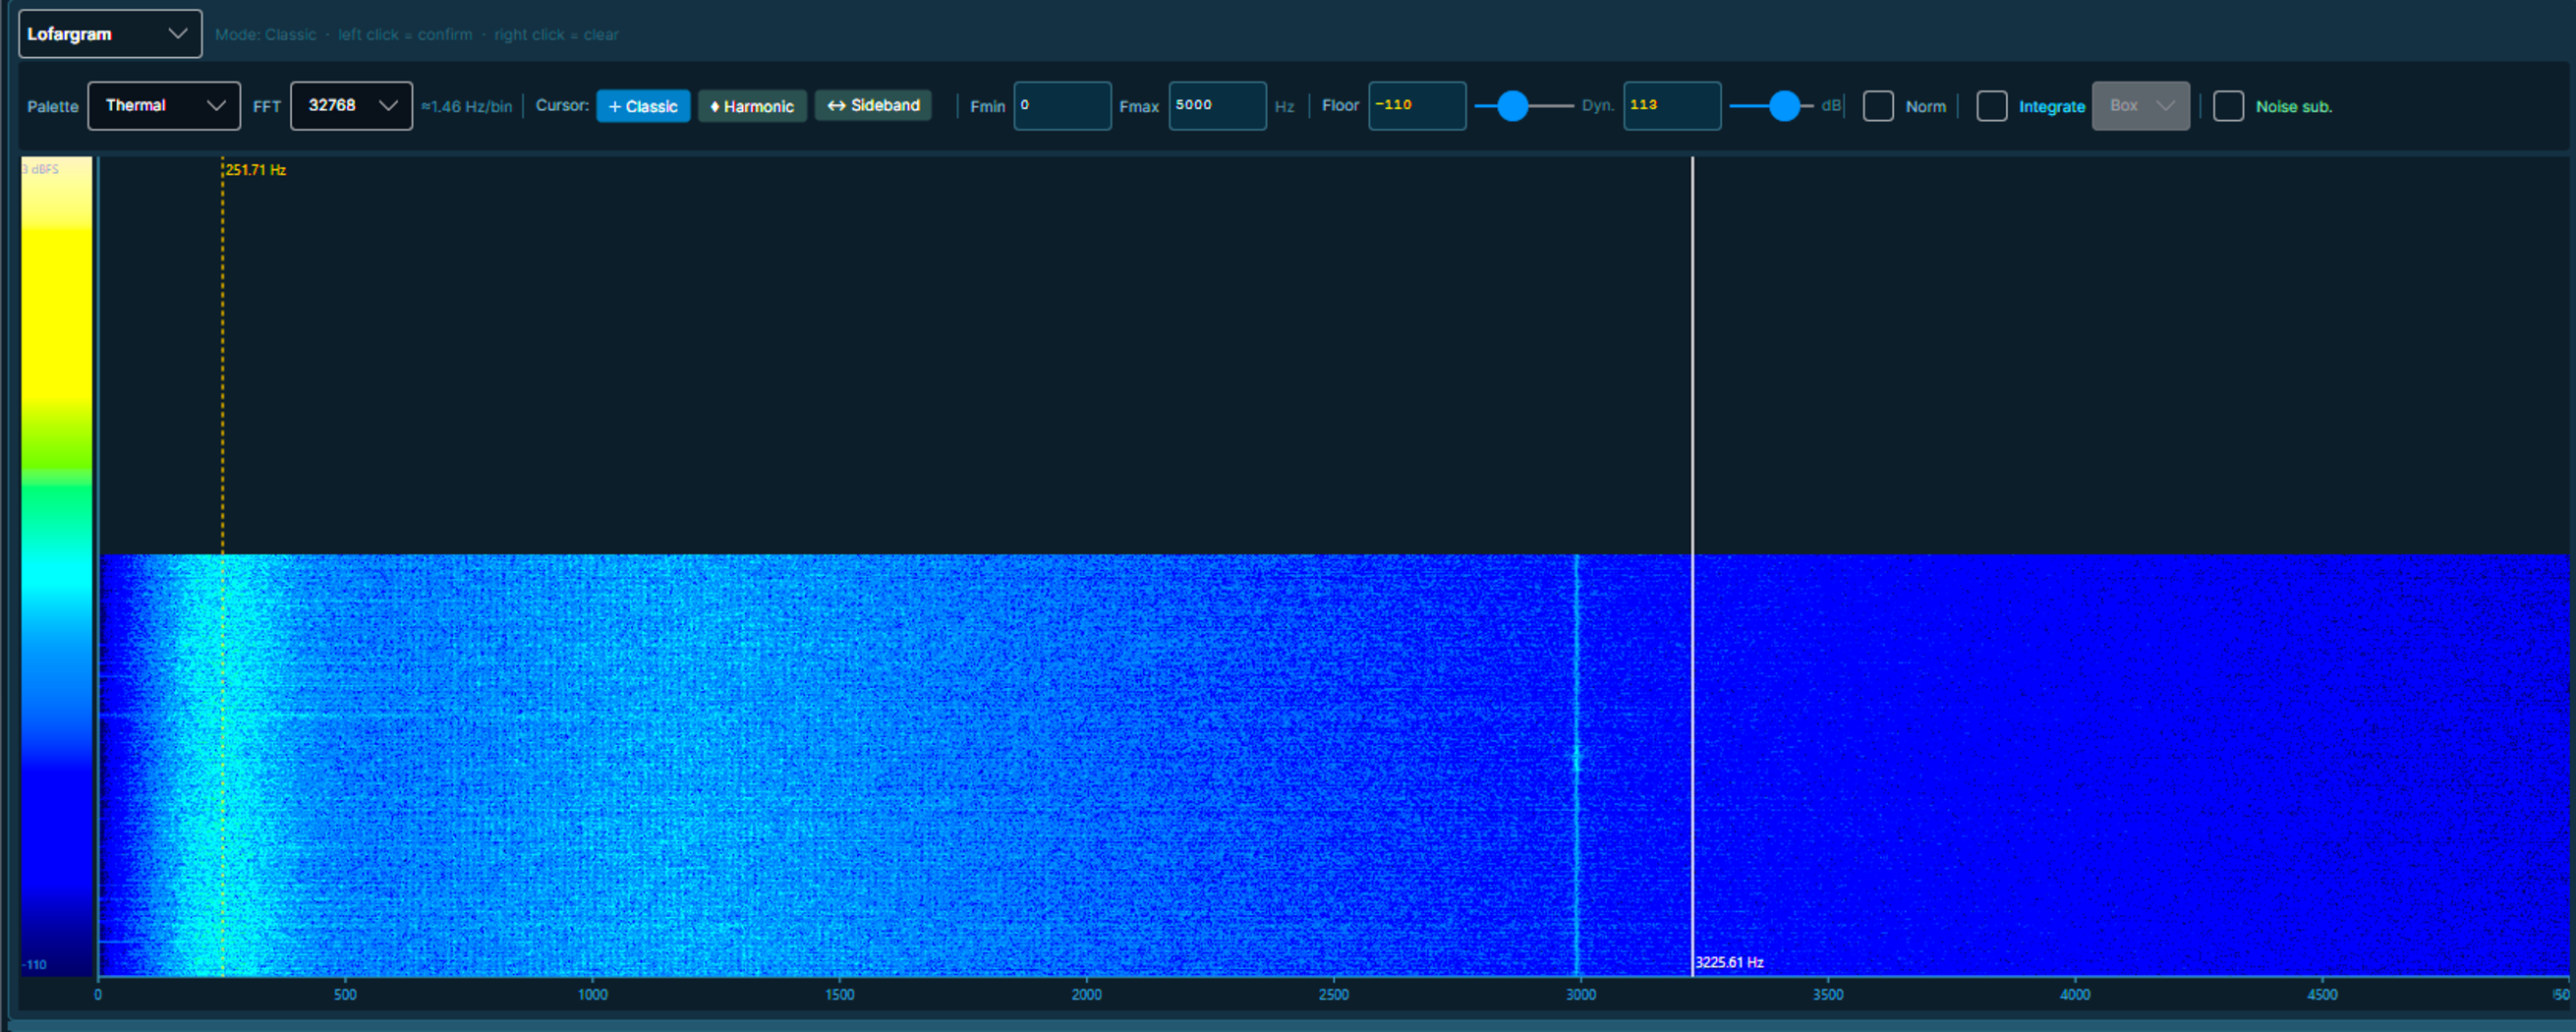
\includegraphics[width=400px]{../img/actuals/panel_A.pdf}
	\caption{Sub-panel A showing a LOFARgram}
\end{figure}

\begin{figure}[h]
	\centering
	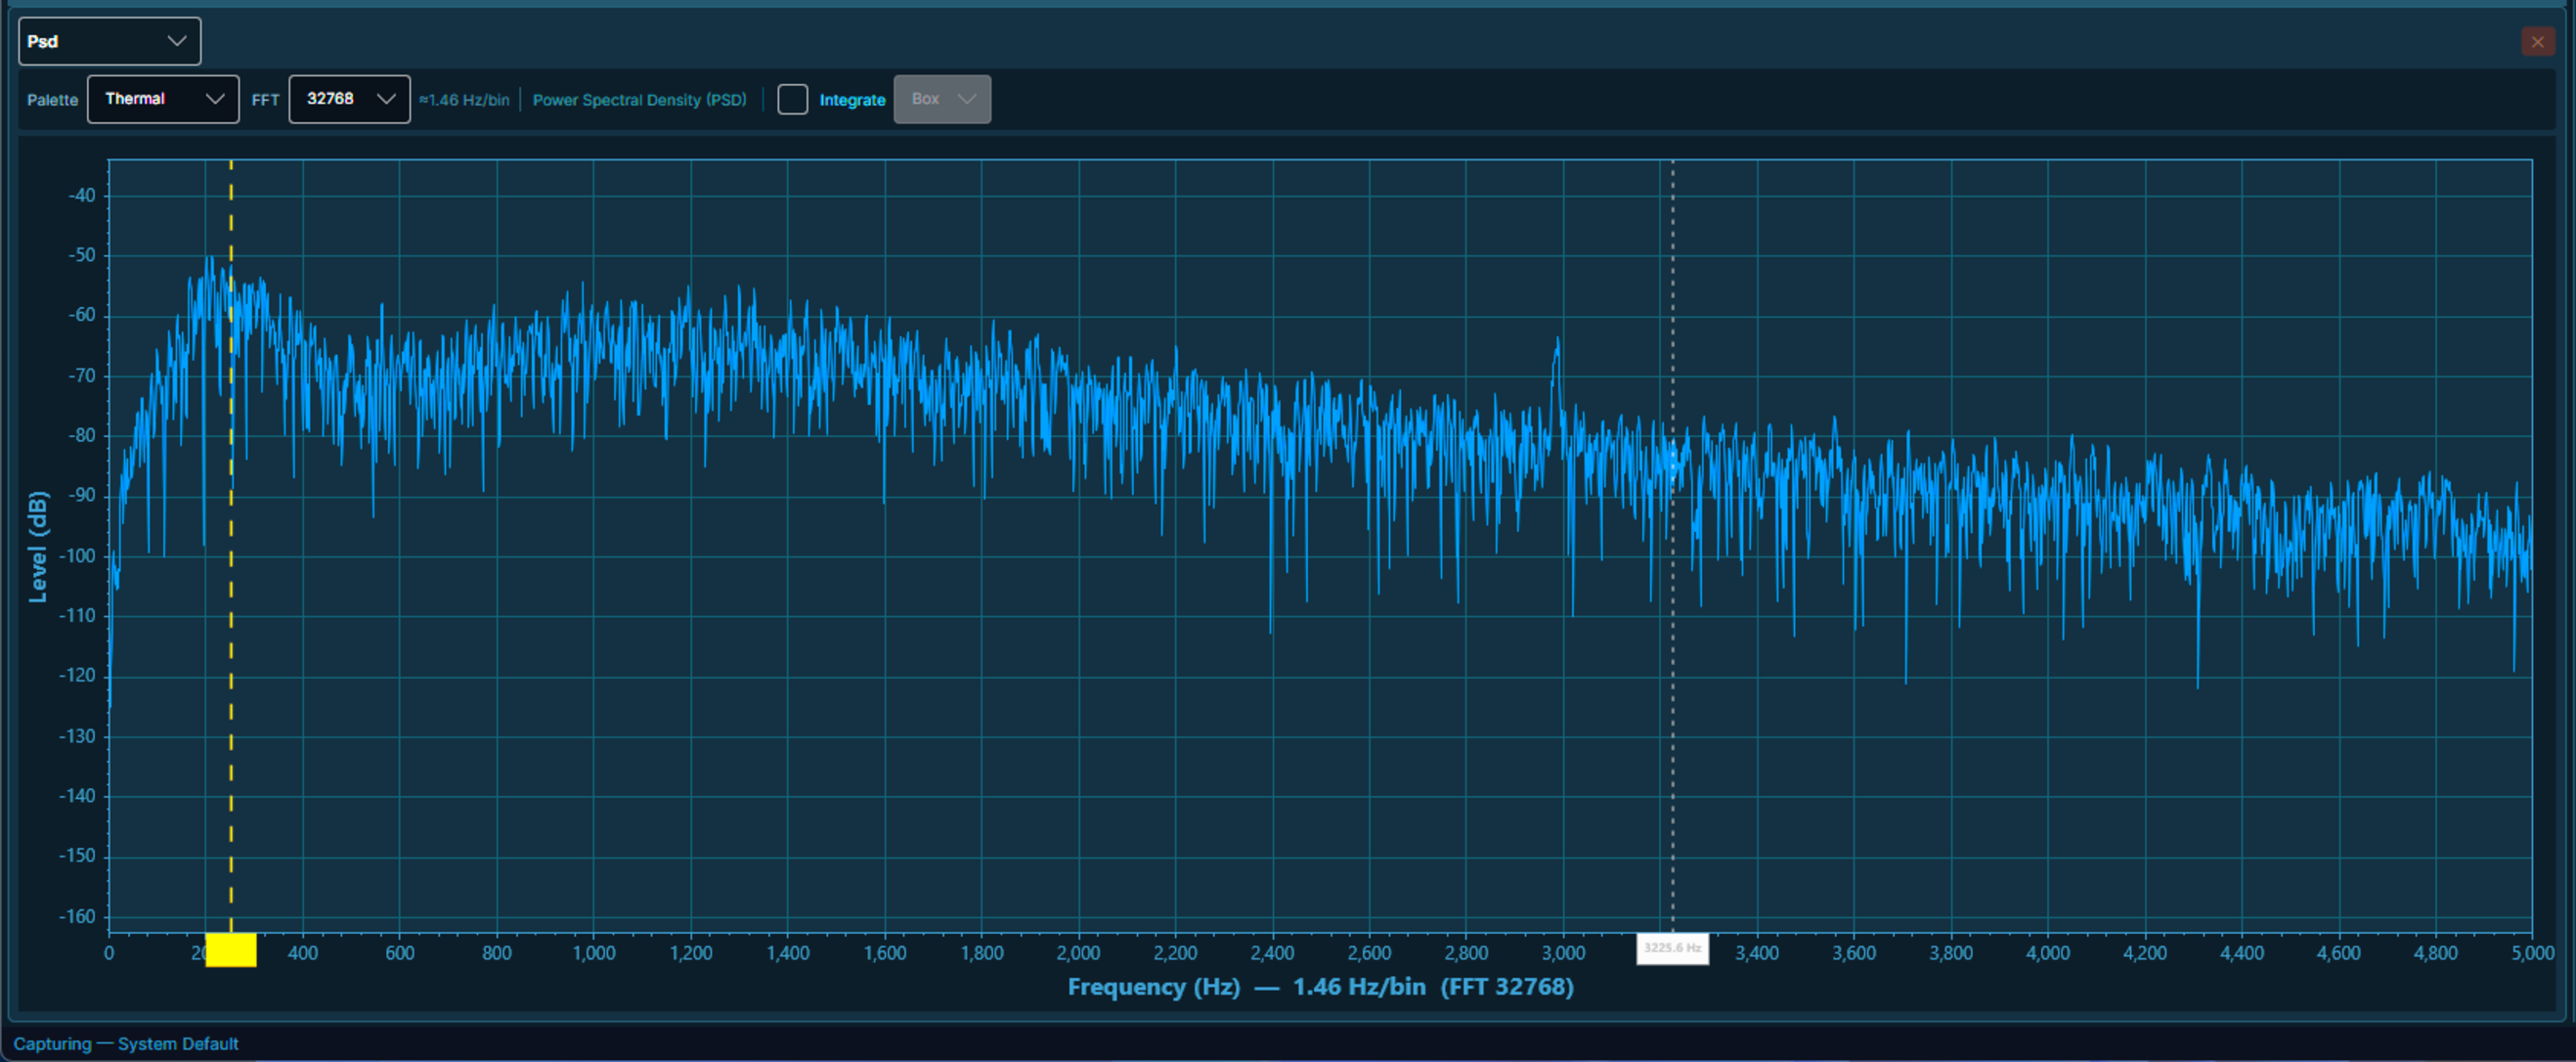
\includegraphics[width=400px]{../img/actuals/panel_B.pdf} % \textwidth
	\caption{Sub-panel B showing the Psd display}
\end{figure}

Each display type has a toolbar with controls specific to its content type. These appear above the panel's display area.

\subsubsection{LOFARgram / DEMON toolbar}
\textcolor{commentGreen}{*** WIP ***}

\textbf{LOFARgram:}

\begin{compactitem}
    \item Palette: Colour palette for the waterfall display. The default is a perceptually uniform palette (Viridis) which is good for visualising low SNR signals.
    \item FFT Size: Number of FFT points (before zero-padding). Larger = better frequency resolution, slower time resolution. Powers of 2: 4096 $\rightarrow$  131072 with $\approx$ 0.34 Hz Bins.
    \item Cursor: Classic, Harmonic and Sideband modes. Shows the current cursor position in time / order and frequency.  Classic shows the cursor position in time and frequency. Harmonic mode shows the cursor position in time and shaft rate (Hz) and displays the harmonic series of the current cursor position. Sideband shows the sidebands either side of the target tonal with their separation in Hz. The cursor can be moved by clicking on the waterfall or by dragging the cursor marker.
    \item $F_{min}$ / $F_{max}$: Display frequency limits (Hz). Crops the visible axis without affecting the pipeline.
    \item Floor (dB): The amplitude level that maps to the coldest colour. Signals below this are clipped to black.
    \item Dyn (dB): Dynamic range: the amplitude span from Floor to the hottest colour. Floor + Dyn = the level that maps to maximum brightness.
    \item Floor slider: Coarse adjustment for Floor.
    \item Dyn slider: Coarse adjustment for Dynamic Range.
    \item Normalisation: Adjusts the waterfall display to compensate for the frequency response of the capture device. See Appendix B for more information.
    \item Integrate: Integration across the live frames improves Signal to Noise Ratio (SNR). Best used for loitering or slow moving targets as moving targets will smear rather than sharpen.
    \item Noise Subtraction: Subtracts a reference noise profile from the waterfall. \textcolor{commentGreen}{*** WIP ***}
\end{compactitem}

\textbf{DEMON:}

\begin{compactitem}
    \item Palette: As for LOFARgram
    \item FFT Size: As for LOFAR but restricted range 256 $\rightarrow$ 4096 with $\approx$ 0.12 Hz Bins.
    \item Cursor: Classic and Harmonic cursor modes. Classic shows the cursor position in time and frequency. Harmonic mode shows the cursor position in time / order and shaft rate (Hz) and displays the harmonic series of the current cursor position.
    \item RPM: Show the cursor frequency in RPM
    \item Blades: \textcolor{commentGreen}{*** WIP ***}
    \item Band: The acoustic frequency band fed into the DEMON envelope detector. Narrowing this to a band with strong broadband noise (e.g. 500 - 5000 Hz) improves signal to noise ratio (SNR).
    \item $F_{max}$: Display frequency limits (Hz). Crops the visible axis without affecting the pipeline.
    \item Floor (dB): The amplitude level that maps to the coldest colour. Signals below this are clipped to black.
    \item Dyn (dB): Dynamic range: the amplitude span from Floor to the hottest colour. Floor + Dyn = the level that maps to maximum brightness.
    \item Floor slider: Coarse adjustment for Floor.
    \item Dyn slider: Coarse adjustment for Dynamic Range.
\end{compactitem}

\subsubsection{Cepstrum / ACF toolbar}
\textcolor{commentGreen}{*** WIP ***}

Same controls as above; Fmin / Fmax instead control the quefrency display range in ms.

\subsubsection{Power Spectral Density (PSD)}
\textcolor{commentGreen}{*** WIP ***}
Power Spectral Density (PSD) analysis is a signal-processing technique used to show how the power (or energy) of a signal is distributed across frequency.

In simple terms:
\begin{compactitem}
    \item A time-domain signal shows how a measurement changes with time.
    \item A PSD shows which frequencies contain the most power.
\end{compactitem}

This makes PSD one of the most useful tools for analysing sounds, vibrations, machinery, sonar recordings, and electrical signals.

\subsubsection{ZoomFft}
\textcolor{commentGreen}{*** WIP ***}

ZoomFFT is particularly useful for:
\begin{compactitem}
    \item Resolving closely spaced shaft-rate harmonics
    \item Measuring small frequency shifts due to vessel speed changes
    \item Separating propeller blade-rate sidebands
    \item Examining a narrow cavitation band with much higher resolution than a full-band FFT
\end{compactitem}

\begin{tabularx}{\linewidth}{l X X}
    \toprule
    \textbf{Feature} & \textbf{FFT} & \textbf{ZoomFFT}\\
    \midrule
    Frequency Range & Entire spectrum & Narrow selected band \\
    Computational cost & Higher for fine resolution & Lower \\
    Resolution in region of interest & Requires very long FFT & Very High\\
    Real-time operation & More demanding & Efficient \\
    Requires frequency translation & No & Yes \\
    \bottomrule
\end{tabularx}

Imagine looking at a ship on the horizon. A normal FFT is like viewing the whole sea with your naked eye but a ZoomFFT is like pointing a telescope at just the ship. You do not gain extra information about the rest of the sea, but you see much finer detail where you're looking. For LOFAR analysis, ZoomFFT is often the preferred way to examine a narrow harmonic family (for example around a shaft rate harmonic or blade-pass frequency) without needing an enormous FFT length.

If you are analysing a signal and already have reason to believe that a narrowband component of interest lies near 42 Hz, you could centre a ZoomFFT at 42 Hz to examine that region at finer frequency resolution.

\begin{compactitem}
    \item Harmonic splitting,
    \item Modulation sidebands,
    \item Slight RPM fluctuations,
    \item Blade-pass sidebands.
\end{compactitem}

This often produces much cleaner results than performing an enormous FFT over the entire acoustic band. For machinery diagnostics and marine acoustics, ZoomFFT is essentially a software implementation of a narrowband spectrum analyser.

\subsection{Settings Panel}

\begin{figure}[ht]
	\centering
	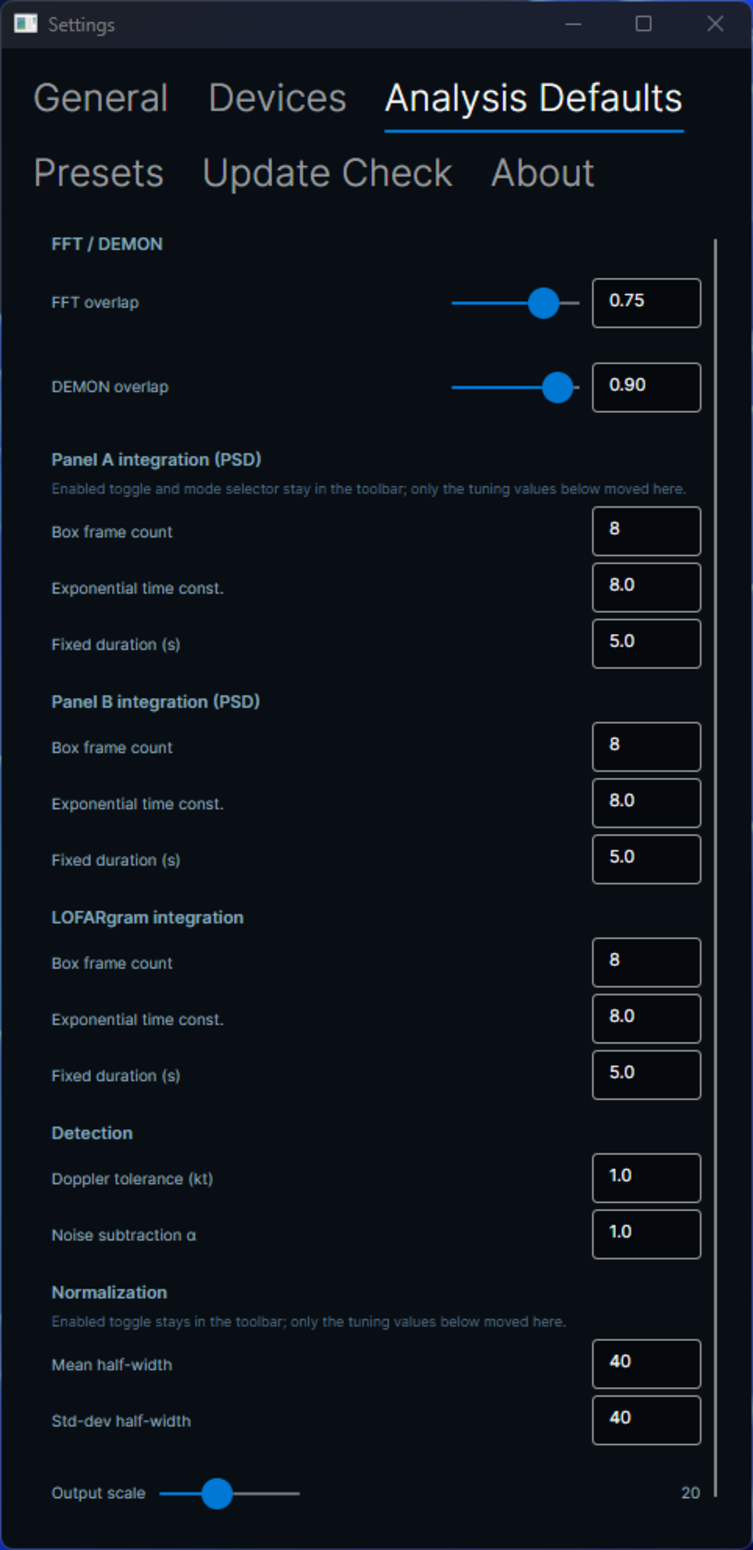
\includegraphics[width=150px]{../img/actuals/analysis.pdf}
	\caption{Analysis Defaults panel}
\end{figure}

Clicking the settings button in the title bar opens a panel with the following control subpages:

\begin{compactitem}
    \item \textbf{General} Allows setting the location of the user recordings folder, defaults to the user's Documents folder.
    \item \textbf{Devices} Sets the sound capture device, the live monitor output device and the recording playback device.
    \item \textbf{Analysis Defaults} Sets FFT / DEMON overlap, panels A/B overlap and integration features (see Figure 5).
    \item \textbf{Presets }Allows user to set up to 5 presets for the analysis parameters (FFT size, overlap, Fmin / Fmax, Floor, Dynamic range, DEMON parameters). Presets are saved to the settings file and restored on next launch.
    \item \textbf{Update Check} Checks for a new version of the application and prompts the user to download it if available.
    \item \textbf{About} View the application version and license information.
\end{compactitem}

\subsection{Right sidebar - Contact Recording and Management}

The right sidebar has two main functions. Capturing and managing contact's sound profiles and matching an unknown sound profile with previously captured ones. It is also used to set up a background sound file which can be used for noise subtraction. Because the use of the contact database and the recording feature is an important part of MACS it has its own section (Section 4).

The right sidebar has a third function, the live monitor. This is a simple audio output of the current capture device. It is useful for checking that the capture device is working and for listening to the sound being captured. The live monitor can be muted or set to a different output device than the capture device.
\pagebreak
\subsection{Noise Subtraction}

In a noisy environment it is often difficult to distinguish potential target tonals from the background. This is often the case in shallow waters. MACS Noise Subtraction allows the user to diminish the effect of this environmental noise. This is achieved by utilizing a pre-recorded sound file of the local environment and then mathematically subtracting it from the live sound. Obviously, this requires that you make a recording of the environment which only has ambient background noise. The mathematical process used is described in detail in Appendix B.

The following steps the user through the process

\begin{compactenum}
    \item Make a recording of the ambient environmental noise and store that for later use. The file must be at least \textbf{15 seconds long} (enforced by validation). Short files produce unstable spectral averages.
    \item When the time comes to use the file select the WAV file that contains \textbf{only ambient/background noise} --- no contact of interest.
    \item Check the \textbf{\enquote{Use as noise reference}} checkbox next to that recording. Only one reference can be active at a time (exclusive selection --- checking one unchecks any previous reference).
    \item Click \textbf{\enquote{Noise sub}} checkbox on the LOFAR panel toolbar to compute and store the reference spectrum.
\end{compactenum}

MACS then attempts to reduce the effect of environment noise which you should observe as the time window progresses.

\begin{advisory}
    \textbf{Note: }The result of noise subtraction can vary due to many confounding factors however it is worth trying if the environment you are operating is particularly noisy. Also noise subtraction will not be effective against some natural sound which have an unpredictable pattern, e.g. whale sounds. More stable natural frequencies such as shrimp may be reduced. That magmatic anomaly will still stand out though. Also noise subtraction may have the unintended effect of hiding the very tonals you are looking for.
\end{advisory}

\subsection{The Cursor System}

The cursor system allows the user to mark individual tonals, identify harmonics and assess sidebands. Select a cursor mode from the toolbar before clicking on the waterfall then click on the tonal you wish to mark.

\begin{compactitem}
\item \textbf{Single:} Places one frequency marker at the clicked frequency $f$.
\item \textbf{Harmonic:} Places harmonic series line starting from the fundamental + N harmonics above it. Configurable N and line width.
\item \textbf{Sideband} Adds sideband lines on both sides of $f$ using the specified spacing $\Delta$ and line count N. "Right only" shows only lines to the right of $f$ (upper sideband).
\end{compactitem}

\subsection{Settings Persistence}

In Windows parameters are saved automatically to \path{C:\Users\%user%\AppData\Roaming\MACS\settings.json}. On Linux and macOS the settings file is located in \path{~/.config/MACS/settings.json}.

This includes: FFT size, overlap, Floor, Dynamic range, Fmin / Fmax, normalisation parameters, DEMON parameters, noise reference path, filter settings, and recordings folder path.

Settings are restored on next launch. If you need to reset to defaults, delete \path{C:\Users\%user%\AppData\Roaming\MACS\settings.json} or \path{~/.config/MACS/settings.json} and restart the application.
\pagebreak